\documentclass{article}
\usepackage{amsmath, tikz, enumerate, sfmath, multicol, tcolorbox}
\renewcommand{\familydefault}{\sfdefault}
\usepackage[top = 0.5in, bottom = 0.5in, left = 1in, right = 1in]{geometry}
\pagestyle{empty}
\raggedright
\tikzset{>=stealth}

\newcounter{example}[section]
\newenvironment{example}[1][]{\refstepcounter{example}\par\medskip
   {\color{red}\textbf{Example~\theexample. #1}}}{\medskip}
\begin{document}


\section*{Vectors: Adding, Subtracting, and Scalar Multiplication}

\begin{tcolorbox}[colframe=orange!70!white, coltitle=black, title=\textbf{Summary}]
\begin{enumerate}
    \item A vector is a directed line segment.
    \item We can add or subtract vectors via corresponding elements if they have the same dimensions and we can multiply any vector by a scalar.
    \item Any 2-dimensional vector can be written in terms of basis vectors $\hat{\imath}$ and $\hat{\jmath}$.
\end{enumerate}
\end{tcolorbox}
% \fbox{\textsc{Today I Can}: Perform arithmetic operations to vectors and matrices.}
\bigskip 

Any point in the coordinate plane can be represented by a directed line segment called a \textbf{vector}. For instance, we can draw a vector from the origin to the point $(3,4)$ below: \newline\\
\begin{center}
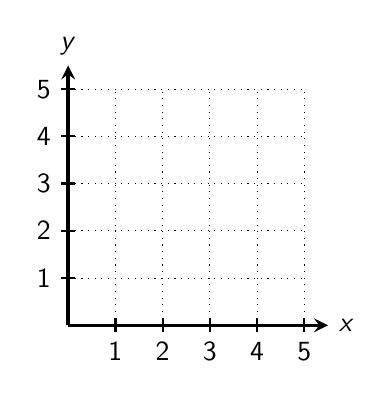
\begin{tikzpicture}[scale=0.6]
\draw[dotted] (0,0) grid (5,5);
\draw[->, very thick] (0,0) -- (5.5,0) node [right] {$x$};
\draw[->, very thick] (0,0) -- (0,5.5) node [above] {$y$};
\foreach \x in {1,2,3,4,5}
\draw [thick] (\x, 0.15) -- (\x, -0.15) node [below] {$\x$};
\foreach \y in {1,2,3,4,5}
\draw [thick] (0.15,\y) -- (-0.15,\y) node [left] {$\y$};
\end{tikzpicture}
\end{center}
\bigskip 

In the above picture, $\vec{v} = \begin{bmatrix}
3 \\ 4
\end{bmatrix}$, where $\vec{v}$ is a \textbf{column vector} with the dimensions 2 rows by 1 column.	\vspace{0.25in}

\emph{Note}: the values in the vector, 3 and 4, are called \textbf{elements}.
\bigskip 

\subsubsection*{Vector Addition}

We can add two vectors together if they have the same dimensions by adding their corresponding elements. \vspace{0.25in}

For instance, suppose $\vec{v} = \begin{bmatrix} 3 \\ 4\\ \end{bmatrix} \text{ and } \vec{w} = \begin{bmatrix} 2 \\ -3 \end{bmatrix}$	\quad then $\vec{v} + \vec{w}$ is
\bigskip 


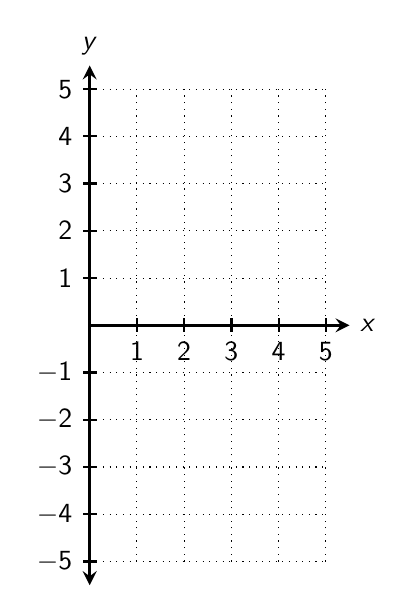
\begin{tikzpicture}[scale=0.6]
\draw[dotted] (0,-5) grid (5,5);
\draw[->, very thick] (0,0) -- (5.5,0) node [right] {$x$};
\draw[<->, very thick] (0,-5.5) -- (0,5.5) node [above] {$y$};
\foreach \x in {1,2,3,4,5}
\draw [thick] (\x, 0.15) -- (\x, -0.15) node [below] {$\x$};
\foreach \y in {-5,...,-1,1,2,...,5}
\draw [thick] (0.15, \y) -- (-0.15, \y) node [left] {$\y$};
\end{tikzpicture}


\newpage

When we physically add vectors, we can move the second vector (without changing its length or direction) so that it starts where the first ends:
\bigskip 

Visually, our previous problem of $\vec{v} = \begin{bmatrix}
3 \\ 4 \end{bmatrix} + \vec{w} = \begin{bmatrix} 2 \\ -3 \end{bmatrix}$ is \vspace{0.25in}

\begin{center}
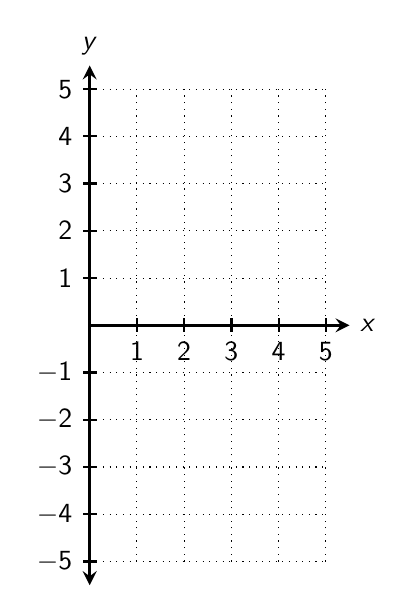
\begin{tikzpicture}[scale=0.6]
\draw[dotted] (0,-5) grid (5,5);
\draw[->, very thick] (0,0) -- (5.5,0) node [right] {$x$};
\draw[<->, very thick] (0,-5.5) -- (0,5.5) node [above] {$y$};
\foreach \x in {1,2,3,4,5}
\draw [thick] (\x, 0.15) -- (\x, -0.15) node [below] {$\x$};
\foreach \y in {-5,...,-1,1,2,...,5}
\draw [thick] (0.15, \y) -- (-0.15, \y) node [left] {$\y$};
\end{tikzpicture}
\end{center}
\bigskip 

\begin{example}
Find and graph the sum of the vectors below.
\[
\vec{v} = \begin{bmatrix}
-1 \\ 3
\end{bmatrix}
\quad \vec{w} = \begin{bmatrix}
-3 \\ 0
\end{bmatrix}
\]
\bigskip

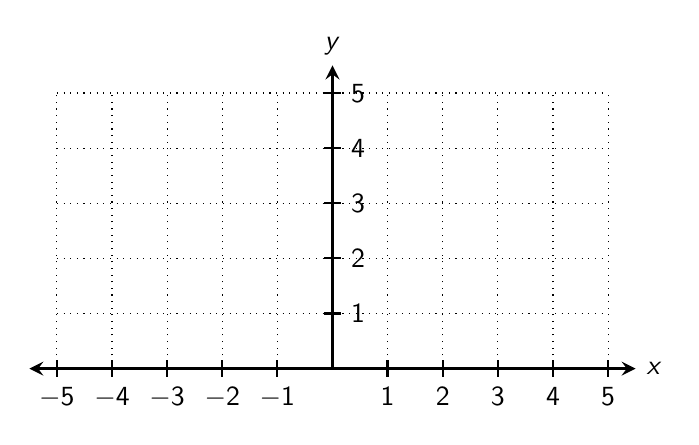
\begin{tikzpicture}[scale=0.7]
\draw[dotted] (-5,0) grid (5,5);
\draw[<->, very thick] (-5.5,0) -- (5.5,0) node [right] {$x$};
\draw[->, very thick] (0,0) -- (0,5.5) node [above] {$y$};
\foreach \x in {-5,...,-1,1,2,...,5}
\draw [thick] (\x, 0.15) -- (\x, -0.15) node [below] {$\x$};
\foreach \y in {1,2,3,4,5}
\draw [thick] (-0.15,\y) -- (0.15,\y) node [right] {$\y$};
\end{tikzpicture}
\end{example}

\newpage
\subsubsection*{Scalar Multiplication}

A \textbf{scalar} is another name for a real number.
\smallskip 

When we multiply a vector by a scale, it scales the vector's length accordingly.	\bigskip 

If $\vec{a} = \begin{bmatrix}
3 \\ -2
\end{bmatrix}$ what is $2\vec{a}\,$? \bigskip

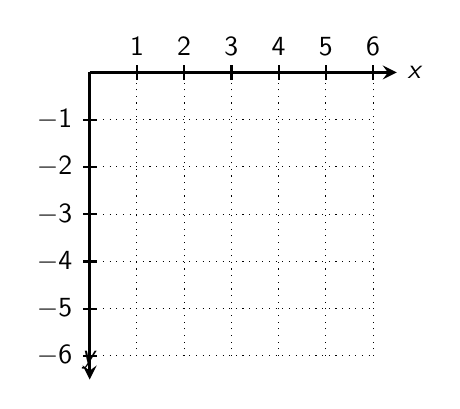
\begin{tikzpicture}[scale=0.6]
\draw[dotted] (0,0) grid (6,-6);
\draw[->, very thick] (0,0) -- (6.5,0) node [right] {$x$};
\draw[->, very thick] (0,0) -- (0,-6.5) node [above] {$y$};
\foreach \x in {1,2,...,6}
\draw [thick] (\x, -0.15) -- (\x, 0.15) node [above] {$\x$};
\foreach \y in {-1,-2,...,-6}
\draw [thick] (0.15,\y) -- (-0.15,\y) node [left] {$\y$};
\end{tikzpicture}

\vspace{0.25in}

What happens when we multiply our vector by $-1$?  \vspace{0.5in}

If $\vec{a} = \begin{bmatrix}
3 \\ -2
\end{bmatrix}$, what is $-1\vec{a}\,$? \bigskip

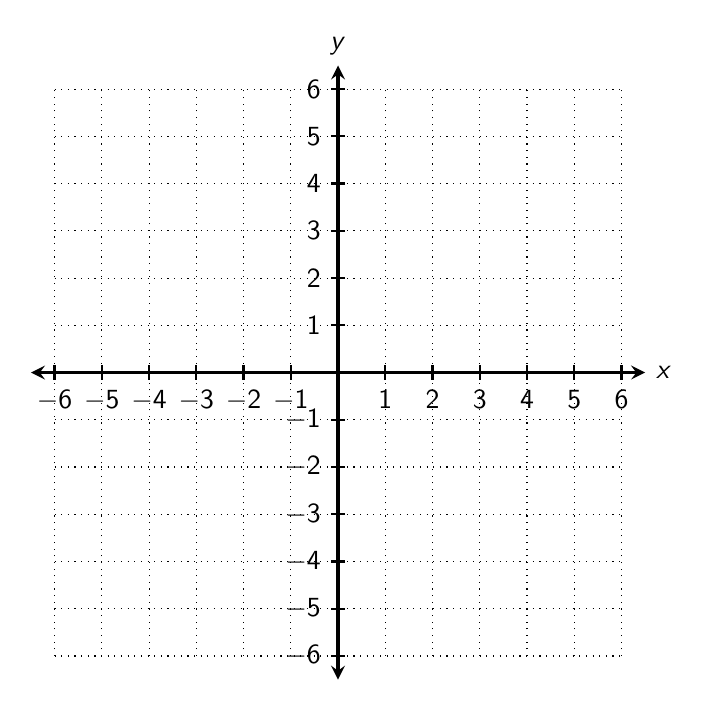
\begin{tikzpicture}[scale=0.6]
\draw[dotted] (-6,-6) grid (6,6);
\draw[<->, very thick] (-6.5,0) -- (6.5,0) node [right] {$x$};
\draw[<->, very thick] (0,-6.5) -- (0,6.5) node [above] {$y$};
\foreach \x in {-6,...,-1,,1,2,...,6}
\draw [thick] (\x, 0.15) -- (\x, -0.15) node [below] {$\x$};
\foreach \y in {-6,...,-1,,1,2,...,6}
\draw [thick] (0.15,\y) -- (-0.15,\y) node [left] {$\y$};
\end{tikzpicture}

\newpage

We can combine the scalar multiples with vector addition.
\bigskip 

\begin{example}
Given $\vec{v} = \begin{bmatrix}
1 \\ -1 
\end{bmatrix}$ and $\vec{w} = \begin{bmatrix}
-2 \\ 0
\end{bmatrix}$ find and graph each.

\begin{enumerate}[(a)]
\begin{multicols}{2}
    \item $\vec{v} - \vec{w}$
    \item $3\vec{v} + \vec{w}$
\end{multicols}
\end{enumerate}
\vspace{0.25in}

\begin{minipage}{0.5\textwidth}
    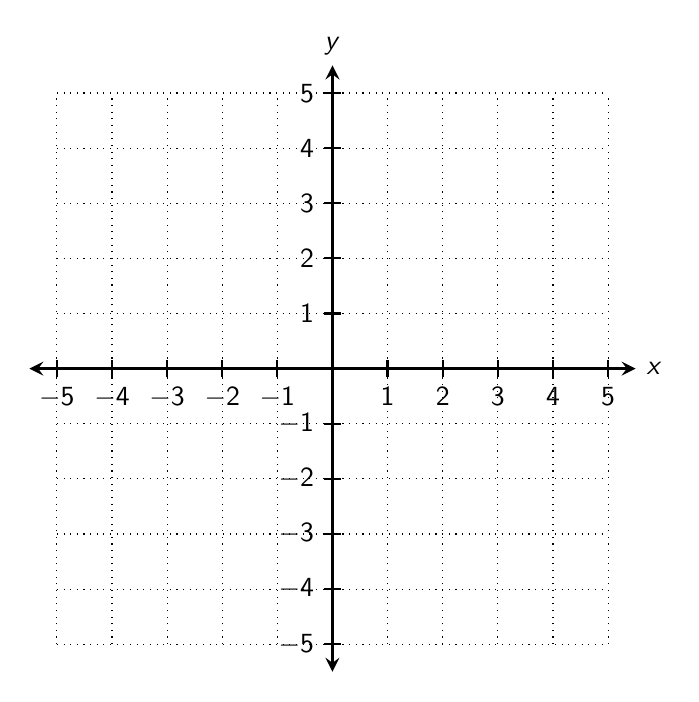
\begin{tikzpicture}[scale=0.7]
    \draw[dotted] (-5,-5) grid (5,5);
    \draw[<->, very thick] (-5.5,0) -- (5.5,0) node [right] {$x$};
    \draw[<->, very thick] (0,-5.5) -- (0,5.5) node [above] {$y$};
    \foreach \x in {-5,...,-1,,1,2,...,5}
    \draw [thick] (\x, 0.15) -- (\x, -0.15) node [below] {$\x$};
    \foreach \y in {-5,...,-1,,1,2,...,5}
    \draw [thick] (0.15,\y) -- (-0.15,\y) node [left] {$\y$};
    \end{tikzpicture}
\end{minipage}
\begin{minipage}{0.45\textwidth}
    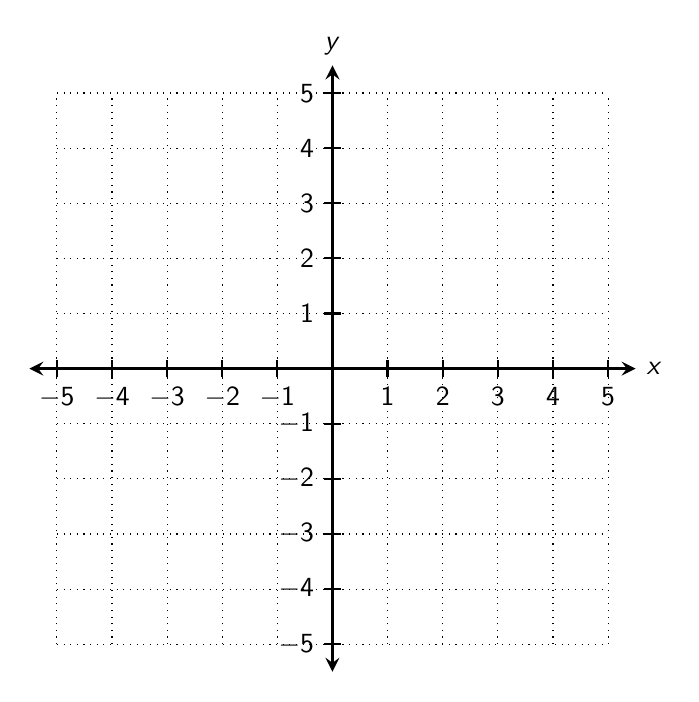
\begin{tikzpicture}[scale=0.7]
    \draw[dotted] (-5,-5) grid (5,5);
    \draw[<->, very thick] (-5.5,0) -- (5.5,0) node [right] {$x$};
    \draw[<->, very thick] (0,-5.5) -- (0,5.5) node [above] {$y$};
    \foreach \x in {-5,...,-1,,1,2,...,5}
    \draw [thick] (\x, 0.15) -- (\x, -0.15) node [below] {$\x$};
    \foreach \y in {-5,...,-1,,1,2,...,5}
    \draw [thick] (0.15,\y) -- (-0.15,\y) node [left] {$\y$};
    \end{tikzpicture}
\end{minipage}
\vfill 
\begin{enumerate}[(a)]  \setcounter{enumi}{2}
    \item $2\vec{v} - 1.5\vec{w}$
\end{enumerate}
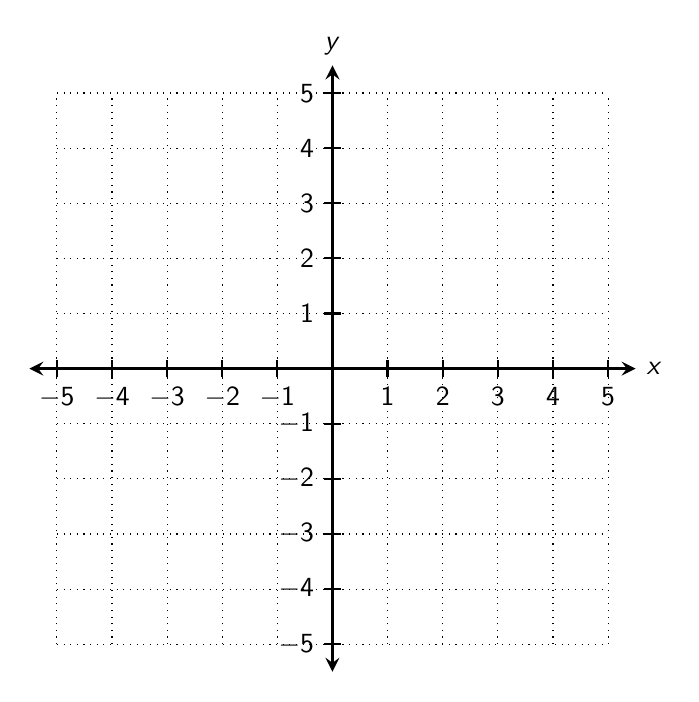
\begin{tikzpicture}[scale=0.7]
    \draw[dotted] (-5,-5) grid (5,5);
    \draw[<->, very thick] (-5.5,0) -- (5.5,0) node [right] {$x$};
    \draw[<->, very thick] (0,-5.5) -- (0,5.5) node [above] {$y$};
    \foreach \x in {-5,...,-1,,1,2,...,5}
    \draw [thick] (\x, 0.15) -- (\x, -0.15) node [below] {$\x$};
    \foreach \y in {-5,...,-1,,1,2,...,5}
    \draw [thick] (0.15,\y) -- (-0.15,\y) node [left] {$\y$};
    \end{tikzpicture}
\end{example}
\vfill 

% (c) \quad $2\vec{v} - 1.5\vec{w}$   \bigskip

% \begin{tikzpicture}[scale=0.7]
% \draw[dotted] (-6,-6) grid (6,6);
% \draw[<->, very thick] (-6.5,0) -- (6.5,0) node [right] {$x$};
% \draw[<->, very thick] (0,-6.5) -- (0,6.5) node [above] {$y$};
% \end{tikzpicture}
% \end{example}


\newpage

\subsubsection*{Basis Vectors ${\pmb{\hat{\imath}}}$ and $\pmb{\hat{\jmath}}$}
\bigskip

The basis vectors $\hat{\imath} = \begin{bmatrix} 1 \\ 0 \end{bmatrix}$ and $\hat{\jmath} = \begin{bmatrix} 0 \\ 1 \end{bmatrix}$ will serve as the foundation for matrix multiplication. \bigskip

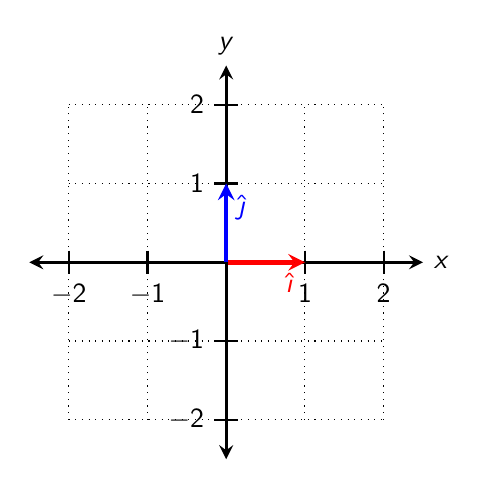
\begin{tikzpicture}[scale=1]
\draw[dotted] (-2,-2) grid (2,2);
\draw[<->, very thick] (-2.5,0) -- (2.5,0) node [right] {$x$};
\foreach \x in {-2,-1,1,2}
\draw [thick] (\x, 0.15) -- (\x, -0.15) node [below] {$\x$};
\draw[->, ultra thick, red] (0,0) -- (1,0) node [below left] {$\hat\imath$};
\draw[<->, very thick] (0,-2.5) -- (0,2.5) node [above] {$y$};
\foreach \y in {-2,-1,1,2}
\draw [thick] (0.15, \y) -- (-0.15, \y) node [left] {$\y$};
\draw[->, ultra thick, blue] (0,0) -- (0,1) node [below right] {$\hat\jmath$};
\end{tikzpicture}
\bigskip 

Any vector can be written as a combination of a scalar and the basis vectors $\hat{\imath} \text{ and } \hat{\jmath}$.
\bigskip 

For instance, $\vec{v} = \begin{bmatrix} 4 \\ 3 \end{bmatrix}$ can be written as follows:	\bigskip

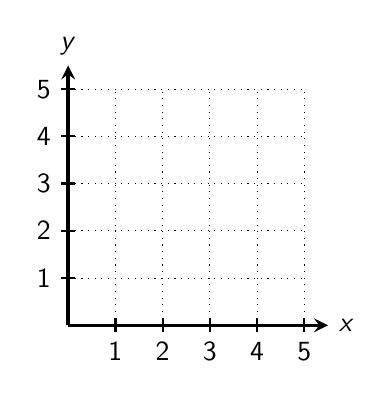
\begin{tikzpicture}[scale=0.6]
\draw[dotted] (0,0) grid (5,5);
\draw[->, very thick] (0,0) -- (5.5,0) node [right] {$x$};
\draw[->, very thick] (0,0) -- (0,5.5) node [above] {$y$};
\foreach \x in {1,2,3,4,5}
\draw [thick] (\x, 0.15) -- (\x, -0.15) node [below] {$\x$};
\foreach \y in {1,2,3,4,5}
\draw [thick] (0.15,\y) -- (-0.15,\y) node [left] {$\y$};
\end{tikzpicture}

\newpage


\begin{example}
Write each in terms of basis vectors $\hat{\imath}$ and $\hat{\jmath}$.  
\begin{enumerate}[(a)]
\begin{multicols}{2}
    \item $\vec{w} = \begin{bmatrix}    -3 \\ 1     \end{bmatrix}$
    \item $\vec{u} = \begin{bmatrix}    5 \\ -2     \end{bmatrix}$
\end{multicols}
\end{enumerate}
\vfill
\begin{enumerate}[(a)]  \setcounter{enumi}{2}
    \item \mbox{} \newline 
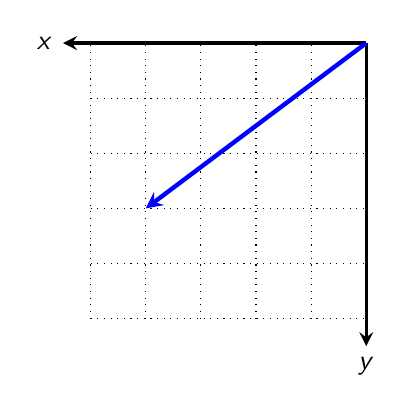
\begin{tikzpicture}[scale=0.7]
\draw[dotted] (-5,-5) grid (0,0);
\draw[->, very thick] (0,0) -- (-5.5,0) node [left] {$x$};
\draw[->, very thick] (0,0) -- (0,-5.5) node [below] {$y$};
\draw[color=blue, ultra thick, ->] (0,0) -- (-4,-3);
\end{tikzpicture}
\end{enumerate}
\end{example}
\vfill
 
\end{document}